\chapter{Introducción específica} % Main chapter title

\label{Chapter2}

%----------------------------------------------------------------------------------------
%	SECTION 1
%----------------------------------------------------------------------------------------

En este capítulo se indican los requerimientos del sistema definidos junto con el cliente y posteriormente se realiza una breve introducción a las tecnologías utilizadas.

\section{Requerimientos}
\label{sec:introducción}

Durante el avance del proyecto surgieron cambios en los requerimientos, algunos sufrieron modificaciones muy pequeñas y se agregaron otros.
Las modificaciones en los requerimientos no generarían atrasos significativos con respecto al tiempo establecido para la finalización del proyecto.

\subsection{Requerimientos del nodo}

\begin{enumerate}
	\item 	Debe tener un relay (5v - 10A) para prender o apagar un dispositivo.
	\item 	Debe tener un módulo LoRa de 915MHz para comunicarse con el gateway.
	\item	Debe medir temperatura ambiente entre 0ºC y 40ºC con un resolución mínima de 8bits.
	\item	Debe tener una fuente switching de pequeño tamaño para suministrar energía a toda la placa del nodo.
	\item	La placa de circuito impreso deberá tener el tamaño tal que pueda ser utilizada en cajas de luz para embutir. Máximo 5x10cm.
	\item	Debe utilizar un led infrarrojo para enviar señales a los aires acondicionados.
	\item	Debe tener un pulsador para cambiar el modo de operación (manual o automático).
\end{enumerate}

\subsection{Requerimientos del gateway}

\begin{enumerate}
	\item	Debe tener un módulo LoRa de 915MHz para comunicarse con los nodos.
	\item	Debe tener conectividad Wi-Fi para comunicarse con el servidor.
	\item	Debe enviar la hora local a los nodos para sincronizar.
	\item	Debe enviar comandos a los nodos.
	\item	Debe tener conexión a un HMI.
\end{enumerate}

\subsection{Requerimientos del servidor}

\begin{enumerate}
	\item	Debe recibir información acerca de los nodos.
	\item	Debe ser accesible a través de una clave encriptada con Hash.
\end{enumerate}

En la figura [\ref{fig:requerimientos2}]se puede ver el sistema planteado para el proyecto con los periféricos mencionados en los requerimientos. En ésta se puede ver la separación entre el nodo y el gateway.

\begin{figure}[ht!]
	\centering
	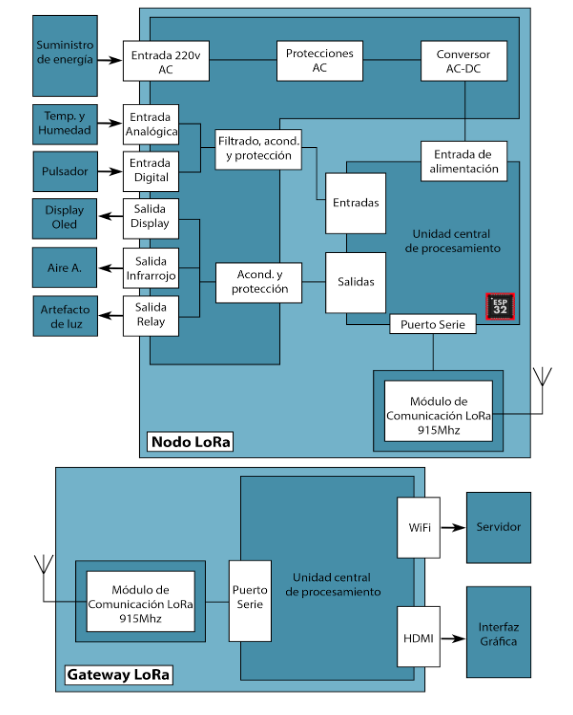
\includegraphics[width=1\textwidth]{./Figures/requerimientos2.png}
	\caption{Esquema general del sistema planteado.}
	\label{fig:requerimientos2}
\end{figure}

\section{Tecnología LoRa}
\label{sec:tecnologialora}

LoRa es un esquema patentado de modulación de espectro ensanchado que deriva de la modulación de espectro ensanchado Chirp (CSS). Establece una relación inversa entre velocidad de datos y sensibilidad dentro de un ancho de banda de canal fijo. Implementa una velocidad de datos variable, utilizando factores de ensanchamiento ortogonales que permiten al diseñador del sistema cambiar la velocidad de datos por rango o potencia, a fin de optimizar el rendimiento de la red en un ancho de banda constante.

LoRa es una implementación de capa física (PHY) y es independiente de las implementaciones de capa superior. Es utilizada en aplicaciones donde se requiere largo
alcance y bajo consumo con ancho de banda limitado, como se indica en la figura [\ref{fig:lora}].

\begin{figure}[ht!]
	\centering
	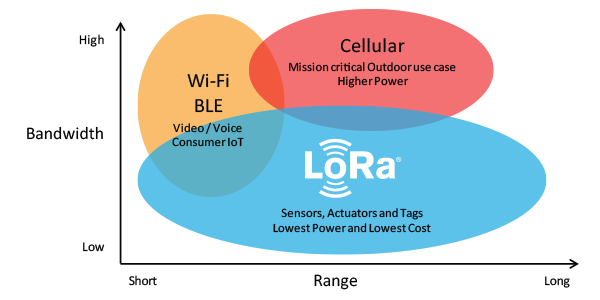
\includegraphics[width=0.8\textwidth]{./Figures/loragrafico.png}
	\caption{Campo de aplicación de tecnología de modulación LoRa.}
	\label{fig:lora}
\end{figure}

A continuación se introducen conceptos y se detallan brevemente las ventajas de la utilización de la tecnología LoRa.

El presupuesto de enlace (link budget) de un sistema o red inalámbrica es una medida de todas las ganancias y pérdidas desde el transmisor, a través del canal de propagación, hasta el receptor objetivo. Estas ganancias y pérdidas incluyen las ganancias y pérdidas del sistema asociadas con la antena, las redes coincidentes, etc., así como las pérdidas del canal de propagación asociado (ya sea a través de datos modelados o medidos).

Se dice que un canal de comunicaciones está limitado por el enlace cuando las pérdidas asociadas con el canal hacen que el nivel de potencia incidente en el receptor sea inferior al requerido para cumplir con el requisito de relación señal ruido (SNR) del receptor para la demodulación correcta de los datos recibidos.

La modulación LoRa es escalable en ancho de banda y frecuencia. Se puede utilizar tanto para salto de frecuencia de banda estrecha como para aplicaciones de secuencia directa de banda ancha. A diferencia de los esquemas de modulación de banda estrecha y banda ancha existentes, LoRa se puede adaptar fácilmente para cualquier modo de operación con solo modificar los registros de configuración del dispositivo.

Al igual que en la modulación por desplazamiento de frecuencia (FSK), LoRa es un esquema de modulación de envolvente constante, lo que significa que las mismas etapas amplificadoras de potencia (PA) de bajo costo y bajo consumo de energía pueden reutilizarse sin modificación. Además, debido a la ganancia de alcance asociada con LoRa, la potencia de salida del transmisor puede reducirse en comparación con un enlace FSK convencional.

Debido a su naturaleza asíncrona, una señal LoRa es muy resistente a los mecanismos de interferencia dentro y fuera de banda. Dado que el período del símbolo LoRa  puede ser más largo que la ráfaga típica de corta duración de los sistemas FHSS de salto rápido, proporciona una excelente inmunidad a los mecanismos de interferencia de AM pulsada. Para una potencia de salida y tasa de transferencia fijas, el presupuesto de enlace de LoRa excede el de FSK. Cuando se toma junto con la robustez probada ante interferencia y desvanecimiento de señal, esta mejora en el presupuesto de enlace puede traducirse fácilmente en un aumento del rango de alcance de más de cuatro veces.

La modulación LoRa emplea factores de ensanchamiento/dispersión ortogonales, lo que permite transmitir múltiples señales de propagación al mismo tiempo y en el mismo canal sin degradación de la sensibilidad de recepción. Las señales moduladas con diferentes factores de dispersión son percibidas como ruido por el receptor y son descartadas.

\section{Planificación}

En la figura [\ref{fig:activityonnode}] se puede ver el Diagrama de {\textit{activity-on-node}} que se presentó en el documento de planificación del proyecto.

\begin{figure}[ht!]
	\centering
	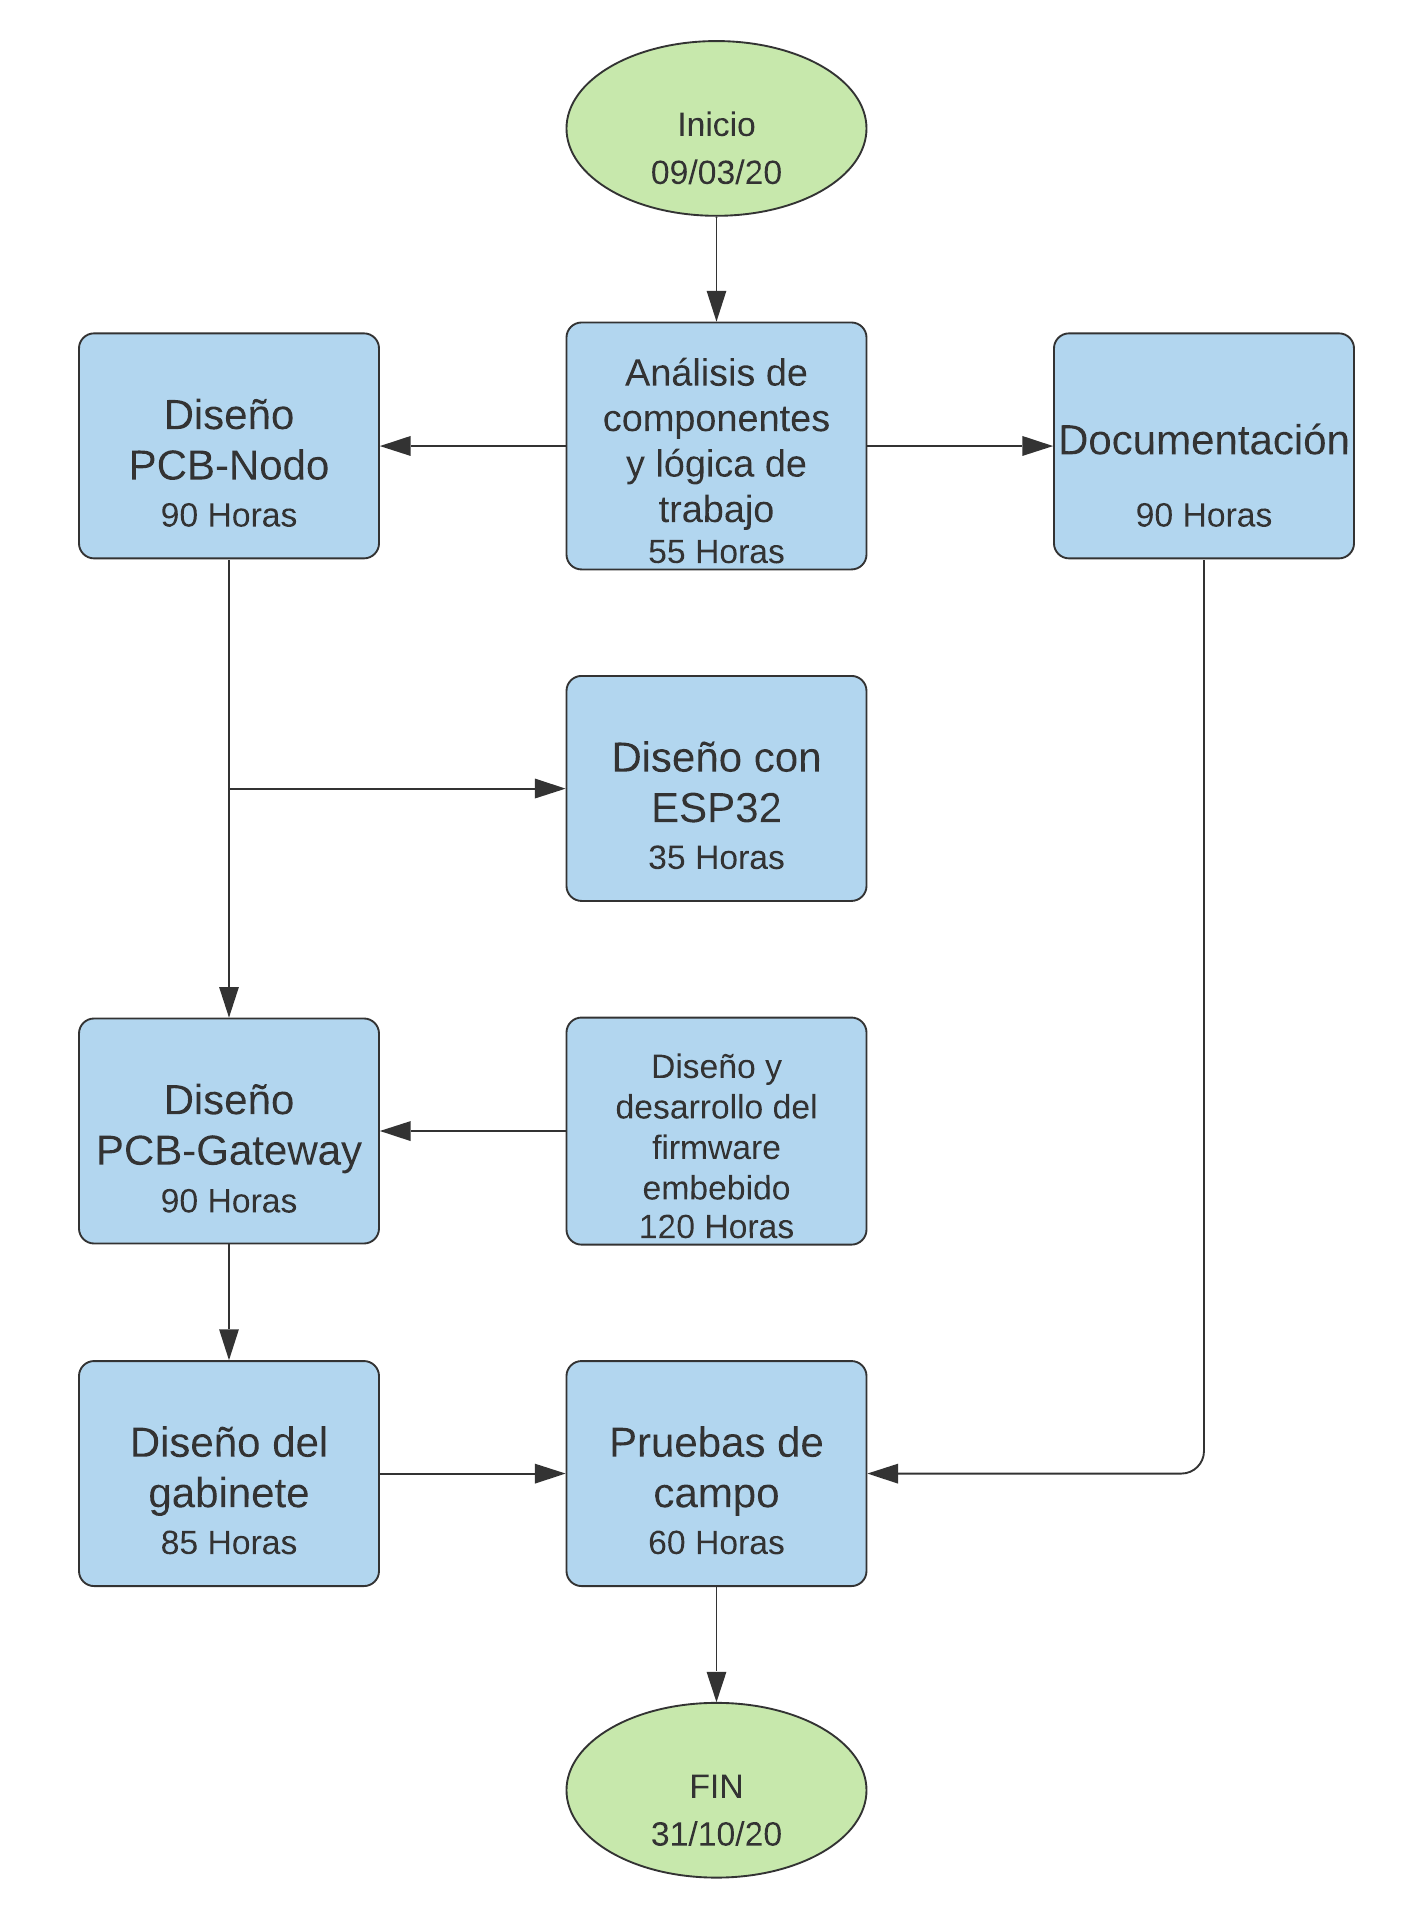
\includegraphics[width=0.8\textwidth]{./Figures/activityonnode.png}
	\caption{Diagrama de {\textit{activity-on-node.}}}
	\label{fig:activityonnode}
\end{figure}

Aquí se pueden ver las tareas a realizar y las horas que se lleva en cada una de las tareas. Cabe resaltar que las horas de la tarea "Diseño del PCB-Gateway" fueron destinadas finalmente al desarrollo del software y firmware del gateway.

